\problemname{Brailleaddition}
För att spara på elräkningarna har Göran bestämt sig för att räkna matematik utan belysning. 
Utan belysning är det svårt att urskilja vanlig text, så därför har Göran bestämt sig för att övergå till Braille (Blindskrift). 
Han behöver nu din hjälp med att verifiera sina uträkningar. 
Skriv ett program som hittar summan av två tal på Brailleform, där asterisk ('*') menar på svart plupp och punkt ('.') menar på vit.

\begin{figure}[h]
    \centering
  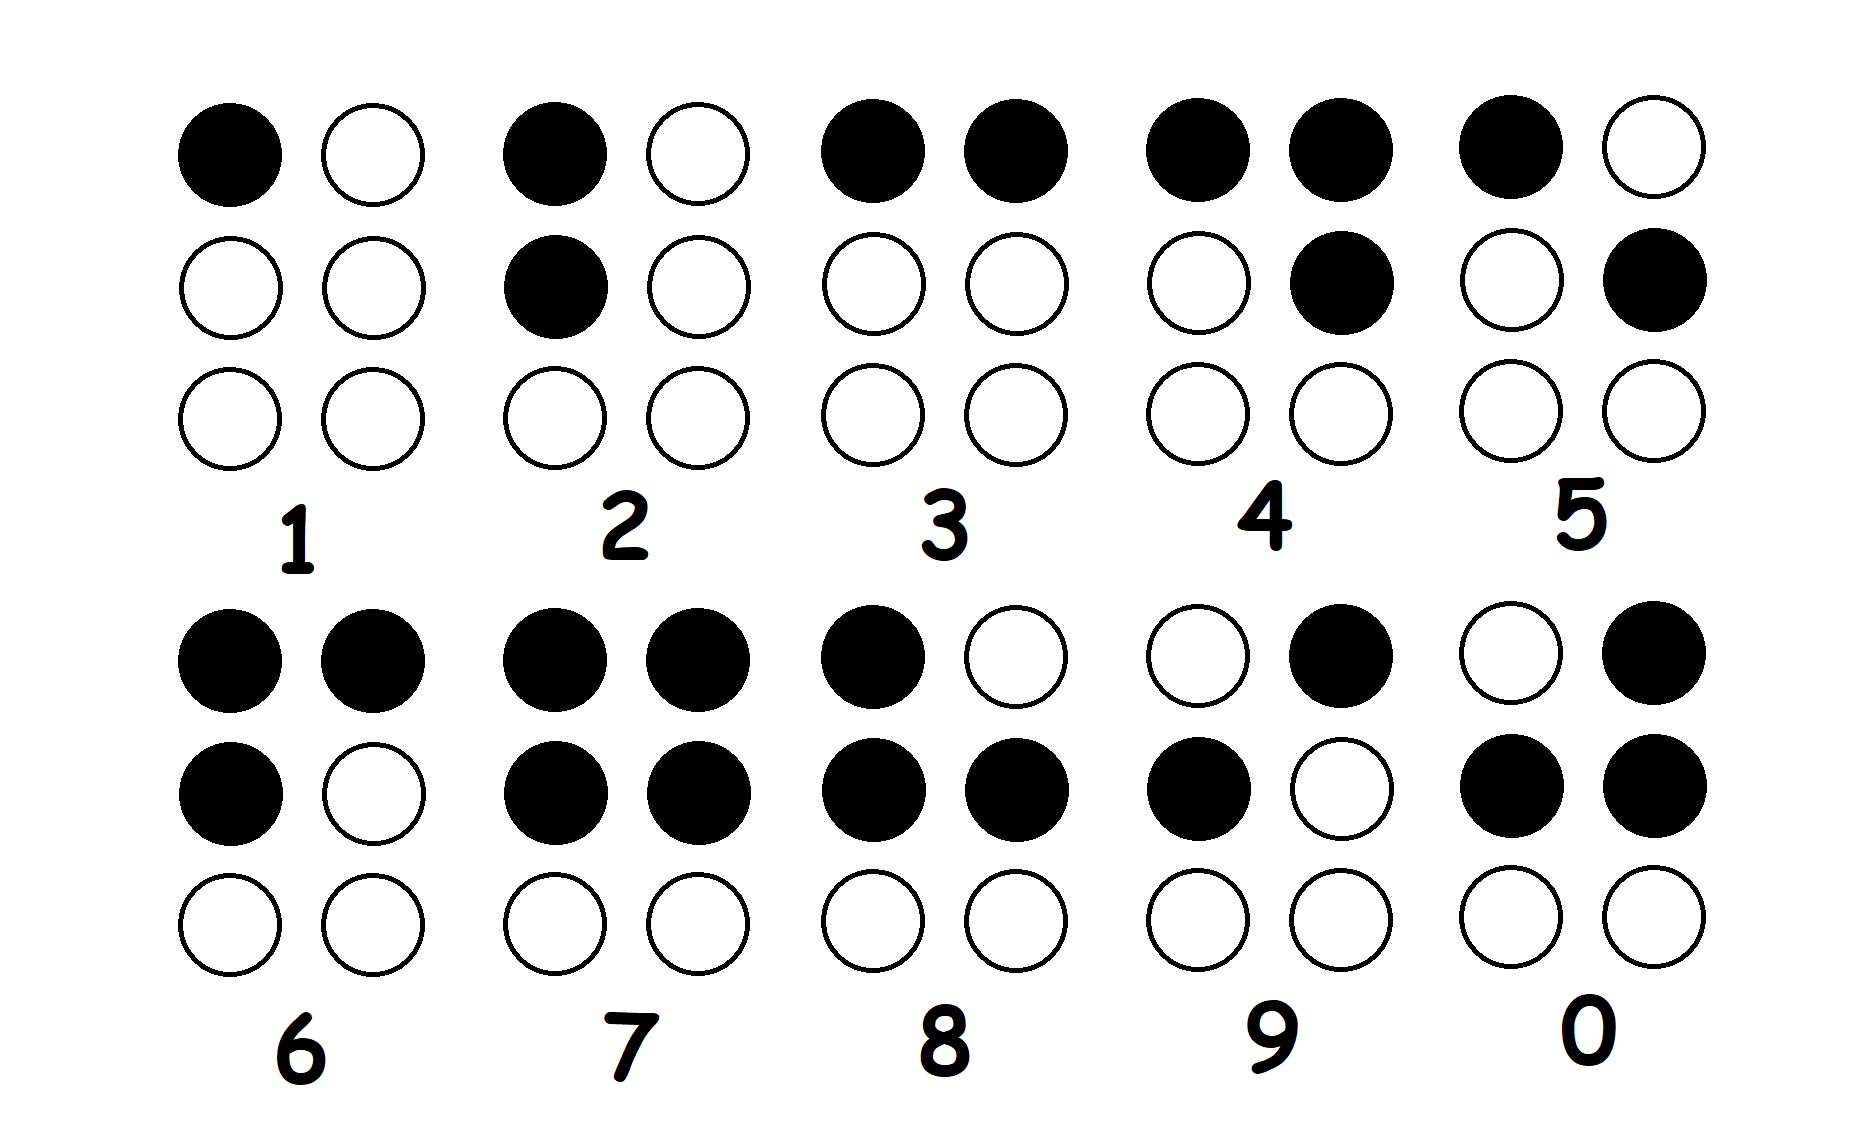
\includegraphics[width=0.75\textwidth]{braille.png}
\caption{Braillesiffrorna 0 till 9.}
\end{figure}

\section*{Indata}
Den första raden innehåller ett heltalen $N$ ($1 \le N \le 9$).

De följande tre raderna innehåller $N$ stycken Braillesiffror som representerar det första talet.

På raden efter kommer ett heltal $M$ ($1 \le M \le 9$). 

De följande tre raderna innehåller $M$ stycken Braillesiffror som representerar det andra talet.

\section*{Utdata}
Mata ut summan av de två talen. Summan ska skrivas med Braillesiffror.

\section*{Poängsättning}
Din lösning kommer att testas på två testfallsgrupper.
För att få poäng för en grupp så måste du klara alla testfall i gruppen.

\noindent
\begin{tabular}{| l | l | p{12cm} |}
  \hline
  \textbf{Grupp} & \textbf{Poäng} & \textbf{Gränser} \\ \hline
  $1$    & $50$      & Enbart braillesiffran ett förekommer. \\ \hline
  $2$    & $50$      & Inga ytterligare begräsningar. \\ \hline
\end{tabular}

\section*{Förklaring av exempelfall}
Det första talet består av Braillesiffrorna $1$, $6$ och $0$ som tillsamman ger talet $160$.
Det andra talet består av Braillesiffrorna $1$ och $6$ som tillsammans ger talet $16$.
Summan ges av $160+16=176$. Summan matas sedan ut med Braillesiffror.